% !TEX root = altosaar-2020-thesis.tex
\chapter{Background}
\label{ch:background}
\lettrine[image=true,lines=3]{design/T}{his} chapter describes probabilistic models and probabilistic inference, taking as examples models from statistical physics and recommender systems.

% !TEX root = ../main.tex
\begin{figure}[t]
  \centering
  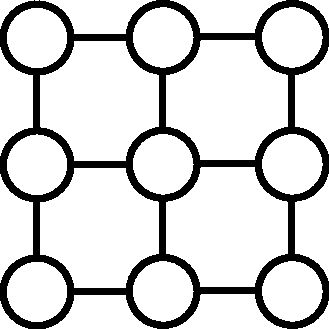
\includegraphics[height=0.2\paperheight]{fig/graphical-model-ising.pdf}
  \caption[Ising model as a probabilistic model]{
  \textbf{The Ising model is a probabilistic model used in statistical physics.} The nodes in this probabilistic graphical model represent random variables, and the edges in the graph represent relationships between neighboring random variables. In this Ising model there are nine random variables variables $\mbz = \{z_1, z_2, \ldots, z_9\}$ represented by nodes and the edges connecting two nodes indicate that those random variables interact in the energy function of the model $E(\mbz)$.}
  \label{fig:graphical-model-ising}
\end{figure}

\section{Probabilistic Models}
Probability models assign probability to configurations of random variables. The random variables in a probability model might correspond to observed variables in a physical system, or to latent properties representing patterns in data collected from the world, or a combination of both. To define a probability model, it is necessary to specify the density $p$ of a collection of random variables $\mbz$. We focus on probabilistic models $p(\mbz)$ where relationships between random variables can be encoded as edges in a graph, or  probabilistic graphical models~\citep{jordan2004graphical}.

\subsection{Example: Ising Model}
\label{sec:ising}
For example, consider a model used in statistical physics: the Ising model. The Ising model can be used to model interactions between atoms in a material~\citep{henelius2016refrustration} to study how the material behaves in different conditions, paving the way toward material design. This probabilistic model has binary random variables $z_n$ with density
\begin{equation}
  p(\mbz; \beta) = \frac{\exp(-\beta E(\mbz))}{\cZ}\, .
  \label{eq:boltzmann}
\end{equation}
The semicolon in \Cref{eq:boltzmann} denotes that the model has a parameter $\beta$, representing the reciprocal temperature of the system of random variables (a physical quantity). The energy function $E(\mbz)$ encodes the relationships between random variables, and $\cZ$, the normalizing constant, ensures that this probability distribution sums to one over all configurations of random variables~\citep{chandler1987introduction}. The energy function of the Ising model is\footnote{Bold letters can denote collections of random variables $\mbz = \{z_1, z_2,...,z_N\}$, or vectors, depending on the context.}
\begin{equation}
\label{eq:ising-energy}
  E(\mbz) = -\frac{1}{2}\sum_{i, j} J_{ij}z_i z_j - H\sum_i z_i\, .
\end{equation}
The interaction strength $J_{ij}$ defines the interactions between random variables. In a simple Ising model, only nearest neighbors interact, so $J_{ij}$ is nonzero if the random variables $z_i$ and $z_j$ are neighbors. The parameter $H$ increases or decreases the energy in proportion to the values of the random variables $z_i$; we give its physical interpretation later.

The Ising model can be represented as a probabilistic graphical model, shown in \Cref{fig:graphical-model-ising}. Two variables $z_i$ and $z_j$ interact (changing the value of one leads to a change in probability of the other) only if they share an edge in the graph. This representation works in conjuction with the density in \Cref{eq:boltzmann}, as the presence of an edge in the graph corresponds to two variables interacting in the energy function $E$. In this model, the energy function (and hence graph) is such that only neighboring random variables interact.

The Ising model can be used to study physical systems such as magnetic materials, where interactions between atoms can be encoded into the interaction strength $J_{ij}$. The interactions between random variables encoded in this manner contain the necessary information to model the properties of a material. In modeling a material, the random variables $\mbz$ can be referred to as spins. Spin is a type of angular momentum carried by particles comprising atoms, and such angular momentum causes a magnetic field. Although the random variables $\mbz$ are binary, taking on values of $-1$ and $+1$, they can be re-scaled to the magnetic strength of the atoms in a particular material of interest if comparison to experimental data is required. The parameter $H$ can be interpreted as the magnitude of an external magnetic field that interacts with the magnetic strength and orientation of every atom~\citep{chandler1987introduction}.

To see how well an Ising model mirrors a physical material, a property such as magnetization can be measured in the material, and calculated using the model. Magnetization is the average orientation of the magnetic strength of every atom or random variable in the material,
\begin{equation}
  M(\mbz) = \frac{1}{N}\sum_{i=1}^N z_i\, .
\end{equation}
By measuring the magnetization $M$ and computing its value in the Ising model, a practitioner can deduce how accurately the model reproduces experimental data. For example, if an Ising model with nearest neighbors ($J_{ij} \neq 0$ if $i$ neighbors $j$) does not accurately reproduce the magnetization of a physical material, it may be necessary to include second-nearest neighbor effects ($J_{ij}\neq 0$ if $i$ and $j$ are connected by a path of length at most two).

Another example of a quantity that can be measured experimentally and computed in a probabilistic model is the thermodynamic free energy $F$,
\begin{equation}
  \label{eq:free-energy}
  F = -\frac{1}{\beta} \log \cZ\, .
\end{equation}
The free energy of a system relates to the amount of energy that can be extracted from a system by its surroundings. For example, the free energy of a protein is used to understand its stability, and can be measured by the amount of energy needed to destroy its structure by denaturing it~\citep{stone2013the-theory}. In modeling a magnetic material or biological material, the free energy can be derived from the normalizing constant $\cZ$~\citep{chandler1987introduction}.

% !TEX root = ../main.tex
\newcommand\x{\scalebox{1.6}{\textbullet}}
\begin{table*}[t]
    \begin{center}
    \resizebox{0.9\textwidth}{!}{%
    \begin{tabular}{@{}lccccccccc|cccccc@{}}
      & \multicolumn{9}{c}{\bf Attributes} & \multicolumn{1}{c}{\bf                                                 User}\\
      \cmidrule(lr){2-10} \cmidrule(lr){11-15}
      {\bf Items} & Pizza & Eggs & Taco & Salad & Avocado & Chicken & Sardines & Beer & Coffee & 1  \\
      Morning Pizza & \x & \x & & & & & & & \x & \x \\
      Dinner Pizza & \x & & & & & & \x & \x & &   \\
      Small Salad & & & & \x & \x & & \x & & &  \\
      Big Salad & & \x & & \x & \x & \x & & & \x & \x  \\
      Taco & & & \x & & \x & \x & & & \x &  \\
      Fish Taco & & & \x & & & & \x & & &  \\
      \bottomrule
    \end{tabular}
    }
    \caption[Example binary classification data]{\label{tab:example-binary}Example binary classification data. A user consumes meals (rightmost column), and meals have attributes (table on the left. Meals are represented as datapoints $x_n$ with covariates being foods in the meals. The goal of a binary classifier trained on this data is to predict which meals a user will consume, or which datapoints $(x_n, y_n)$ have a label $y_n = 1$. An accurate classifier will information about which covariates are shared across positive or negative labeled datapoints; for example, this user consumes meals that include eggs and coffee.
    }
    \end{center}
\end{table*}
\subsection{Example: Binary Classification}
% !TEX root = ../main.tex
\begin{figure}[t]
  \centering
  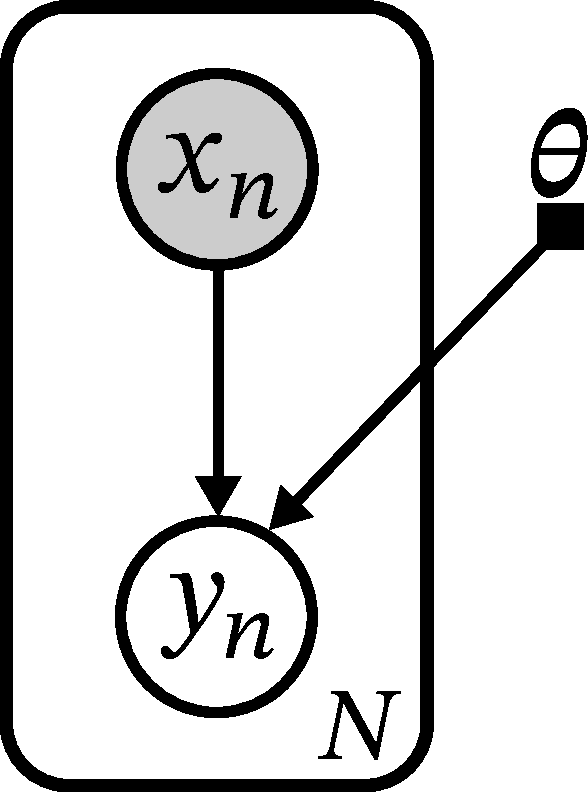
\includegraphics[height=0.2\paperheight]{fig/graphical-model-regression.pdf}
  \caption[Graphical model for logistic regression]{
  \textbf{Binary classification is a probabilistic modeling technique used in recommender systems.} Observed random variables are denoted by shaded nodes, and directed edges in the graph indicated conditional dependence on a node's parents. There are $N$ independent, identically distributed observations $(y_n, x_n)$; the rectangular plate denotes repetition of nodes and edges. The model predicts a binary response $y_n$ using parameters $\mbtheta$ and covariates $x_n$.}
  \label{fig:graphical-model-regression}
\end{figure}
Another example of a probabilistic model is a binary classifier~\citep{bishop2006pattern}, represented as a graphical model in \Cref{fig:graphical-model-regression}. Consider $N$ datapoints of the form $(x_n, y_n)$ consisting of covariates $x_n$ and binary responses $y_n$. As illustrated in \Cref{tab:example-binary}, the covariates $x_n$ might represent information about items such as foods in a meal, and $y_n$ may indicate whether a single user ate a meal with those foods. A binary classifier would then classify whether the user would eat a new meal $\hat{x}_n$ based on its constituent foods.

A binary classifier is defined using a regression function $f$ with parameters $\mbtheta$. The logistic function $\sigma$ applied to the regression function defines the probability model for a binary classifier,
\begin{equation}
  p(y_n \mid x_n; \mbtheta) = \frac{\exp\left( \sigma(f(x_n; \mbtheta)) \cdot y_n\right)}{\cZ}\, .
  \label{eq:binary-classification}
\end{equation}
The logistic function constrains the output of $f$ to the unit interval, and $\cZ$ is again the normalizing constant. The regression function $f$ uses information about a datapoint to classify whether the response $y_n$ is positive. An example of a regression function is an inner product, defined by
\begin{equation}
  f(x_n; \mbtheta) = \mbtheta^\top x_n\, ,
\end{equation}
which corresponds to logistic regression~\citep{bishop2006pattern}. Alternatively, a more flexible model can be built using a deep neural network~\citep{lecun2015deep}.
%A binary classifier can form the basis of a recommender system as we study in \Cref{ch:rfs}.

\section{Inference}
In a probability model, computing---or, inferring---properties of the probability distribution is a central task. One inference problem is to ascertain likely configurations of random variables. Another is to compute the sum of a probability distribution over a set of random variables, for example, to compute the normalizing constant~\citep{jordan2004graphical}.

\subsection{Computing Likely Configurations of Random Variables}
In the study of a probability model such as a binary classifier in \Cref{eq:binary-classification}, one question of interest is: for a set of observations $(x_n, y_n)$, what is a likely value of $\theta$? Maximum likelihood estimation is one way to answer this question~\citep{bishop2006pattern}.

A probability distribution like $p(\mby \mid \mbx; \mbtheta)$ is also known as a likelihood function. It defines the likelihood of a random variable $\mby$ conditional on the value of data $\mbx$, with the current setting of the parameters $\mbtheta$. The maximum likelihood estimate of the parameters of this probability model for the data $(\mbx, \mby)$ is given by
\begin{equation}
  \mbtheta^* = \argmax_{\mbtheta} p(\mby \mid \mbx; \mbtheta)\, .
\end{equation}
This maximum likelihood estimate of the parameters $\mbtheta^*$ can be computed using stochastic optimization if the data is large~\citep{robbins1951a-stochastic}. % what if the argmax is intractable, or an integral? #todo details

\subsection{Computing the Normalizing Constant}

The second central inference task in probabilistic modeling is summing a probability model over a set of random variables. One example of this is computing the normalizing constant $\cZ$. This inference problem requires computing a sum: the normalizing constant ensures a probability distribution sums to $1$ over values the random variables can take.

Consider computing the normalizing constant for the binary classifier in \Cref{eq:binary-classification}.  To compute the normalizing constant $\cZ$ for this probability model, we can sum over the binary values the random variable $y_n$ can take,
\begin{align}
1 &= \sum_{y_n \in \{0, 1\}} \frac{\exp\left( \sigma(f(x_n; \mbtheta)) \cdot y_n\right)}{\cZ} \\
\Rightarrow \cZ &= \sum_{y_n \in \{0, 1\}} \exp\left( \sigma(f(x_n; \mbtheta) \cdot y_n)\right)\\
\cZ &= 1 + \exp\left( \sigma(f(x_n; \mbtheta))\right)\, .
\end{align}
Inference of the normalizing constant $\cZ$ is straightforward in this probability model. The random variable $y_n$ is binary, so there are only two terms in the sum needed to compute the normalizing constant.

Next, consider computing the normalizing constant or partition function for the Ising model in \Cref{eq:boltzmann}. The random variables $z_n$ in this model also take on binary values. The partition function is computed by summing over all the values associated with all random variables in the system, $\mbz = \{z_1, \ldots, z_N\}$:
\begin{align}
1 &= \sum_{z_1 \in \{-1, +1\}} \ldots \sum_{z_N \in \{-1, +1\}} \frac{\exp(-\beta E(\mbz))}{\cZ}\\
\Rightarrow \cZ &= \sum_{z_1 \in \{-1, +1\}} \ldots \sum_{z_N \in \{-1, +1\}} \exp(-\beta E(\mbz))\, .
\label{eq:intractable-partition}
\end{align}
There are $N$ binary-valued random variables and $2^N$ terms in the sum required to compute the partition function, so inference in the Ising model is difficult. For Ising models used to study materials, the partition function is intractable to compute for most model sizes practitioners want to study and compare to physical realizations.

One way to address the issue of an intractable partition function is with sampling methods, such as Markov chain Monte Carlo~\citep{metropolis1953equation}. These algorithms enable inference by simulating likely configurations of random variables. These samples of likely configurations are used to approximate quantities of interest such as the partition function. But, Markov chain Monte Carlo methods are difficult to scale to probabilistic models with large numbers of correlated random variables. In this thesis, we instead use variational inference, an approximate inference algorithm that relies on optimization instead of sampling.
% Calculating the partition function can be difficult, and there are many ways around computing the partition function. For example, sampling methods and variational methods can be used to approximate properties of distributions such as properties derived from the partition function. Markov chain Monte Carlo~\citep{metropolis1953equation} allows sampling system configurations from the Boltzmann distribution of a model; these samples can be used to approximate physical quantities. Variational inference relies on optimizing (varying) functionals to derive approximations of distributions of interest, these approximations can be used to compute properties of a model. Variational inference has roots in mean field methods in physics~\citep{saul1996mean,hoffman2013stochastic,blei2017variational} as described in \Cref{ch:background}.

\section{Variational Inference}
% !TEX root = ../main.tex
\begin{figure}[t]
  \centering
  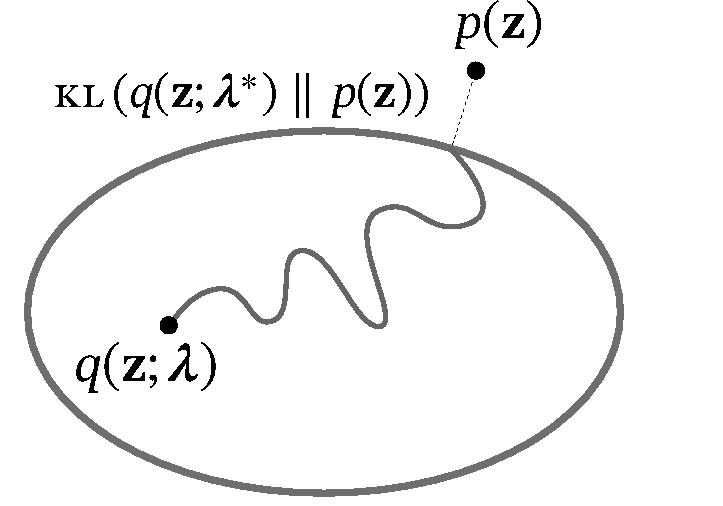
\includegraphics[height=0.2\paperheight]{fig/vi-cartoon.pdf}
  \caption[Variational inference cartoon]{
  \textbf{Variational inference finds the member of the variational family closest to the target distribution.} The oval in the cartoon represents the space of variational approximations $q(\mbz; \mblambda)$, and the goal of \acrlong{vi} is to find variational parameters $\mblambda^*$ that yield an approximation close to the target probability model $p(\mbz)$. One way to measure the distance between a variational approximation and the target probability distribution is with the \gls{kl} divergence.}
  \label{fig:vi-cartoon}
\end{figure}
Instead of working with a probability model $p(\mbz)$ directly, \acrfull{vi} posits a family of distributions $q(\mbz; \mblambda)$ indexed by parameters $\mblambda$~\citep{blei2017variational}. The goal of \gls{vi} is to find the closest member of the variational family $q$ to the target distribution $p$. The algorithm consists of varying the parameters $\mblambda$ to improve the quality of the approximation, as illustrated in \Cref{fig:vi-cartoon}. One way to measure the distance between the variational approximation and the target distribution is with the \acrfull{kl} divergence, or relative entropy~\citep{mackay2003information,ranganath2018black}.

The intractable partition function in $p(\mbz)$ appears in the \gls{kl} divergence \gls{vi} uses to assess distance,
\begin{equation}
\label{eq:kl}
    \KL{q(\mbz; \mblambda)}{p(\mbz)} = \E_q[\log q(\mbz ; \mblambda)] -\E_q[\log p(\mbz)] \\
\end{equation}
But it is possible to derive an objective function that does not depend on the partition function, starting from the \gls{kl} divergence. Taking the Ising model in \Cref{eq:boltzmann} as an example,
\begin{align}
  \KL{q(\mbz; \mblambda)}{p(\mbz)} &= \E_q[\log q(\mbz ; \mblambda)] -\E_q[\log p(\mbz)] \\
 \KL{q(\mbz; \mblambda)}{p(\mbz)} &= \E_q[\log q(\mbz ; \mblambda)] -\E_q[-\beta E(\mbz) - \log \cZ] \\
 \log \cZ &= \E_q[-\beta E(\mbz)] - \E_q[\log q(\mbz ; \mblambda)] + \KL{q(\mbz; \mblambda)}{p(\mbz)} \label{eq:second-last}  \\
 \Rightarrow \log \cZ \geq \cL(\mblambda) &\coloneq  \E_q[-\beta E(\mbz)] - \E_q[\log q(\mbz ; \mblambda)]\, .
 \label{eq:llbo}
\end{align}
This lower bound $\cL$ on the log normalizing constant is also called the \acrfull{elbo}, and serves as the objective function for \gls{vi}. In deriving this lower bound from \Cref{eq:second-last} to \Cref{eq:llbo}, we used the fact that the \gls{kl} is greater than or equal to zero. To show this fact, we start from Jensen's inequality for a convex function $f$, or
\begin{equation}
  f(\E[\mbz]) \leq \E[f(\mbz)]\, .
\end{equation}
The logarithm in the \gls{kl} is concave, so its negative is convex. We apply Jensen's inequality to the negative \gls{kl} in \Cref{eq:kl}:
\begin{align}
  -\KL{q(\mbz)}{p(\mbz)} &= \E_q\left[\log \frac{p(\mbz)}{q(\mbz )}\right] \\
  &\leq \log \E_q\left[\frac{p(\mbz)}{q(\mbz )}\right]\\
  &= \log \int  q(\mbz) \frac{p(\mbz)}{q(\mbz )}d\mbz \\
  &= \log \int  p(\mbz)d\mbz \\
  &= 0 \, .
\end{align}
This shows that the \gls{kl} is greater than or equal to zero~\citep{cover2012elements}.

The left-hand-side in \Cref{eq:llbo} does not change as the variational parameters $\mblambda$ are varied in $\cL(\mblambda)$. In words, maximizing the lower bound $\cL(\mblambda)$ is equivalent to minimizing the \gls{kl} divergence between the variational approximation and target probability model.

\subsection{Example: Mean Field Variational Inference in the Ising model}
\label{sec:ising-mean-field}

To demonstrate \gls{vi}, we use the Ising model described in \Cref{sec:ising} with probability distribution $p(\mbz)$ defined in \Cref{eq:boltzmann} and energy function $E(\mbz)$ in \Cref{eq:ising-energy}. Inspecting the intractable partition function of the Ising model can help construct a variational family $q(\mbz; \mblambda)$ to approximate the Ising model.

The Ising model partition function in \Cref{eq:intractable-partition} is intractable because the sums do not decompose by random variables: every sum must be carried out in order, because the result of the $N$th sum over the random variable $z_N$ depends on the results of the sums over the previous $N-1$ random variables. This is because of interactions between dependent random variables. The first term in the energy function of the Ising model represents nearest neighbor interactions, $z_iz_j$, and is graphically equivalent to the links between nearest neighbors in \Cref{fig:graphical-model-ising}.

However, the second term in the Ising energy function in \Cref{eq:ising-energy}, $H\sum_i z_i$, does decompose by random variable. Physically, this corresponds to a magnetic field applied to the system as a whole, so every random variable is subject to the same force. Mathematically, there is an outer sum over every configuration of random variables, and in this term the results of the summation over a variable $z_i$ do not affect the summation over another variable $z_j$. So this magnetic field term can be evaluated for systems with many random variables.

% !TEX root = ../main.tex
\begin{figure}[t]
  \centering
  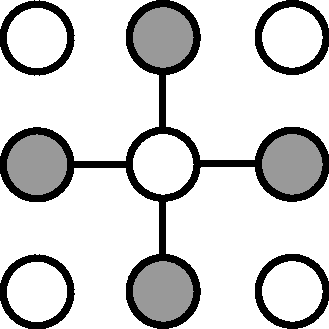
\includegraphics[height=0.2\paperheight]{fig/ising-markov-blanket.pdf}
  \caption[Markov blanket of a node in an Ising model]{
  \textbf{The structure of an Ising model can inform variational approximations.} This graphical model illustrates a Markov blanket in the Ising model of \Cref{fig:graphical-model-ising}. The Markov blanket of a node is the set of nodes whose values need to be fixed to render a node independent of the rest of the graph. In an Ising model, only neighboring random variables interact and therefore comprise the Markov blanket of a node. Here, the Markov blanket of the central node are shaded, indicating that their values are fixed. The missing edges between the peripheral nodes indicate that the central node is independent of the rest of the graph, conditional on its Markov blanket.}
  \label{fig:ising-markov-blanket}
\end{figure}
The structure of the Ising model energy function and corresponding graphical model can be used to build a variational approximation $q(\mbz; \mblambda)$ as follows. If the second term of the Ising model energy function does not lead to an intractable partition function due to every random variable being subject to a magnetic field, one can construct a variational approximation by extending this physical intuition and developing the concept of a `mean field'. Consider the central random variable $z_i$ in \Cref{fig:graphical-model-ising}. Fixing the values of its nearest neighbors renders this random variable independent of the rest of the graph as shown in \Cref{fig:markov-blanket-ising}. The nearest neighbors of the central random variable can then be interpreted as giving rise to a magnetic field. The strength of this magnetic field is unknown, so we can define this unknown strength as a variational parameter $\delta H$ that we will infer using \gls{vi}. This mean field is additive to the external magnetic field $H$ applied to the system as a whole, so the energy function for the central random variable $z_i$ under this mean field assumption can be written
\begin{equation}
  E_{\mf}(z_i; \delta H) = \delta H z_i + H z_i\, .
\end{equation}
Note that we have replaced the interaction term $J_{ij} z_iz_j$ in the Ising model energy function in \Cref{eq:ising-energy} by the mean field $\delta H$. The mean field assumption is that term can approximate the effects of neighboring nodes~\citep{chandler1987introduction}. If we repeat this argument for every node in the graph, we arrive at the mean field energy function
\begin{equation}
  E_{\mf}(\mbz; \delta H) = -(H + \delta H)\sum_{i = 1}^N z_i\, .
  \label{eq:mean-field-energy}
\end{equation}
The above construction starting from the mean field assumption corresponds to the variational approximation with density
\begin{equation}
  q(\mbz; \beta, \delta H) = \prod_{i=1}^N\frac{\exp(- \beta E_\mf(z_i; \delta H))}{\cZ_\mf} \, ,
  \label{eq:mean-field-distribution}
\end{equation}
and we see that the variational parameter $\mblambda$ is simply the mean field strength $\delta H$. The mean field variational approximation corresponds to a fully factorized probability distribution where every random variable is independent~\citep{wainwright2008graphical}. This is a useful property, as the partition function is tractable in this mean field variational approximation: we can compute the partition function for every random variable by itself. The partition function for a single random variable $z_i$ under the mean field assumption is straightforward,
\begin{align}
  \cZ_\textrm{\mf, i} &= \sum_{z_i \in \{-1, +1\}} \exp(- \beta (H + \delta H) z_i) \\
  &= 2 \cosh (\beta (H + \delta H)) \, ,
  \label{eq:partition-function-i}
\end{align}
and the partition function for the variational approximation for all variables is simply $\cZ_\mf = \cZ_\textrm{\mf, i}^N$. Similarly, the average of a random variable under the variational distribution is readily computed as
\begin{align}
\begin{split}
  \E_{q(z_i)}[z_i] &= \sum_{z_i \in \{-1, +1\}} \frac{z_i \exp(- \beta E_\mf(z_i; \delta H))}{\cZ_\textrm{\mf, i}} \\
 &= \sum_{z_i \in \{-1, +1\}} \frac{z_i \exp(- \beta (H + \delta H) z_i)}{2 \cosh(\beta (H + \delta H))} \\
 &= -\tanh(\beta (H + \delta H))\, .
 \label{eq:mf-mean}
 \end{split}
\end{align}
Now that we have constructed a variational family for the Ising model, we can proceed with the \gls{vi} algorithm. The next step is writing down and maximizing the lower bound on the log partition function to minimize the \gls{kl} between our approximating distribution and model.

The lower bound on the log partition function $\cL(\delta H)$  in \Cref{eq:llbo} becomes
\begin{align}
  \cL(\delta H) &= \E_q[-\beta E(\mbz)] - \E_q[\log q(\mbz; \delta H)] \\
  &= \E_q\left[-\frac{1}{2}\beta\sum_{i, j} J_{ij}z_i z_j - \beta H\sum_i z_i\right] - \E_q\left[ -\beta (H + \delta H)\sum z_i\right] + \log \cZ_{\mf} \\
  &= \E_q\left[-\frac{1}{2}\beta\sum_{i, j} J_{ij}z_i z_j + \beta\delta H\sum_i z_i\right] + \log \cZ_{\mf}\, ,
\intertext{and we can take the expectation inside the sum using the fact that the mean field variational distribution is fully factorized, so }
  \cL(\delta H) &= -\frac{1}{2}\beta \sum_{i, j}J_{ij}\E_{q(z_i)}[z_i]\E_{q(z_j)}[z_j] + \beta \delta H \sum_i \E_{q(z_i)} [z_i] + \log \cZ_{\mf}\, .\\
\end{align}
In the first term, recall that two random variables $z_i$ and $z_j$ have the same distribution under the mean field assumption, and that every variable interacts with its four nearest neighbors in the Ising model. The lower bound on the log partition function then becomes
\begin{align}
 \cL(\delta H) &= -\frac{1} {2} \beta 4JN \E_{q(z_i)}[z_i]^2 + \beta N \delta H \E_{q(z_i)} [z_i] + \log \cZ_{\mf}\, .
\end{align}
The next step in the \gls{vi} algorithm is maximizing this lower bound, to minimize the \gls{kl} divergence between the variational approximation and the model. Taking the derivative with respect to $\delta H$ and suppressing the subscript of the expectation operator, we get
\begin{align}
\frac{\partial\cL(\delta H)}{\partial \delta H} &= N\beta(-4J\E[z_i]\partial_{\delta H}\E[z_i] + \E[z_i] + \delta H \partial_{\delta H} \E[z_i]) + N\beta \tanh(\beta (H + \delta H))\, .
\end{align}
Next, setting this derivative to zero and cancelling out terms (and using \Cref{eq:mf-mean}) leads to
\begin{align}
 0 &= -4J\E[z_i]\partial_{\delta H}\E[z_i] + \delta H \partial_{\delta H} \E[z_i]) \\
 \Rightarrow \delta H \partial_{\delta H} \E[z_i]) &= 4J\E[z_i]\partial_{\delta H}\E[z_i] \\
 \Rightarrow \delta H^* &= 4J\E[z_i]\, .
\end{align}
This shows that under a mean field assumption, the variational parameter that maximizes the lower bound on the log partition function---and hence minimizes the \gls{kl} divergence between the approximation and model---is proportional to the mean field around any node in the system. The structure of the model informs our choice of variational approximation.

The quality of the variational approximation $q(\mbz; \beta, \delta H^*)$ from \gls{vi} can be assessed in several ways. For example, the magnetization $M$ or the free energy $F$ can be calculated using the variational approximation, and these values can be compared to Markov Chain Monte Carlo simulations in small systems. This can be viewed as a type of predictive check for a \gls{vi} algorithm~\citep{blei2014build}. However, the development of theoretical guarantees to assess the quality of variational approximations found with \gls{vi} is an open area of research~\citep{wang2019frequentist}. Practitioners must currently empirically evaluate the quality of variational approximations according to the task at hand, as we do in \Cref{ch:hvm,ch:pvi}.

\subsection{Variational Inference Originated in Statistical Physics}

Previously, we derived a variational approximation to the Ising model by making a mean field assumption. That the language of physics is used in machine learning algorithms such as \gls{vi} is no coincidence. In fact, \citet{feynman1972statistical,feynman2018statistical} derives the \gls{gbf} inequality for use in a variational principle for approximating intractable partition functions using mean field assumptions. Consider a model with energy function $E$ and partition function $\cZ$, and a mean field variational approximation with energy function $E_\mf$ (and corresponding partition function $\cZ_\mf$). Then the \gls{gbf} inequality reads~\citep{feynman1972statistical,feynman2018statistical}
\begin{equation}
\cZ \geq \cZ_\mf\exp\left(-\beta \braket{E - E_\mf}_\mf\right) \, .
\label{eq:gbf-inequality}
\end{equation}
In physics, bra-ket notation is used to denote expectations. For example, expectations with respect to \Cref{eq:mean-field-distribution} are written $\braket{\; \cdot \;}_\mf$. Rewriting the \gls{gbf} with statistics notation for the expectation $\E_q[\;\cdot\;]$ yields
\begin{align}
 \cZ &\geq \cZ_\mf\exp\left(-\beta \E_q[E - E_\mf]\right) \, .
\end{align}
Taking the logarithm, we recover the lower bound on the log partition function
\begin{align}
 \log \cZ &\geq \E_q[-\beta E] - \E_q[-\beta E_\mf] + \log \cZ_\mf\\
 &= \E_q[-\beta E] - \E_q[\log q_\mf(\mbz; \mblambda)] \\
 &= \cL(\mblambda)\, .
\end{align}
This is identical to the log partition function lower bound in \Cref{eq:llbo}. \citet{hoffman2013stochastic} review the historical roots of the variational principle in its machine learning incarnation.

To complete the connection to machine learning, we relate this log partition function lower bound to the evidence lower bound studied in the \gls{vi} literature~\citep{blei2017variational}. A probabilistic model of data might have the following process for generating data $\mbx$ using prior information in latent variables $\mbz$:
\begin{align*}
\mbz &\sim p(\mbz)\\
\mbx &\sim p(\mbx \mid \mbz)
\end{align*}
The posterior distribution of this model is computed using Bayes' rule,
\begin{equation*}
  p(\mbz \mid \mbx) = \frac{p(\mbx \mid \mbz) p(\mbz)}{p(\mbx)} \, .
\end{equation*}
The model evidence $p(\mbx)$ is the partition function of the posterior. Calculating the partition function is what makes posterior inference difficult, as it requires integration over the latent variables $\mbz$,
\begin{equation*}
  p(\mbx) = \int p(\mbx, \mbz) d\mbz \, ,
\end{equation*}
and the latent variables $\mbz$ are typically high-dimensional, such as the number of random variables in an Ising model. But \gls{vi} can be used to approximate this intractable integral. The lower bound on the log partition function becomes the \gls{elbo}:
\begin{align}
\log p(\mbx) &\geq \cL(\mblambda) \\
\cL(\mblambda) &= \E_q[\log p(\mbx, \mbz)] - \E_q[\log q(\mbz ; \mblambda)] \, .
\end{align}
An example of a latent variable model without data is the Ising model---in this case, the data is an empty set, $\mbx = \{\}$. In this case $\cL(\mblambda)$ is a lower bound on the log partition function as we derived in \Cref{eq:llbo} and identical to the \gls{gbf} inequality.
% \gls{vi} is an algorithm to find a good approximation to a target probability distribution that has an intractable integral, such as the sum needed to compute a partition function. We now turn to the second inference problem of computing likely configurations of variables in a probability model.

\section{Conclusion}
We reviewed probability models and gave examples of their use in statistical physics and recommender systems. The task of inference is central to working with probability models; we described variational inference and maximum likelihood estimation. The following chapters address the issue of building the structure of a problem into a performant probability model, whether that structure concerns the connectivity in a statistical physics model, the structure of datapoints in a recommender system, or information about a variational approximation useful in an optimization algorithm for this approximation.